% Notes and solutions


% -------------------------------------------------
% Package imports
% -------------------------------------------------
\documentclass[12pt, a4paper]{article}
\usepackage[utf8]{inputenc}% Input encoding
\usepackage[english]{babel}% Set language to english
\usepackage{graphicx}% For importing graphics
\usepackage{amsthm, amsfonts, amssymb, bm}% All the AMS packages
\usepackage{mathtools}% Fixes a few AMS bugs
\usepackage[expansion=false]{microtype}% Fixes to make typography better
\usepackage{hyperref}% For \href{URL}{text}
\usepackage{fancyhdr}% For fancy headers
\usepackage[sharp]{easylist}% Easy nested lists
\usepackage{parskip}% Web-like paragraphs
\usepackage{multicol}% For multiple columns
\usepackage{tikz-cd}% For diagrams
\usepackage{microtype}
\usepackage{listings}% To include source-code
\usepackage[margin = 2.5cm, includehead]{geometry}% May be used to set margins
\usepackage{nicefrac}% Enables \nicefrac{nom}{denom}
%\usepackage[sc]{mathpazo}% A nice font, alternative to CM
\usepackage{booktabs}
\usepackage{fancyvrb} % fancy verbatim

% -------------------------------------------------
% Package setup
% -------------------------------------------------

\newcommand{\Title}{Solutions to\\``Pattern Recognition and Machine Learning''\\by Bishop}
%\newcommand{\Subtitle}{A summary of main ideas and concepts}
\newcommand{\Author}{\texttt{tommyod} @ github}
\newcommand{\listSpace}{-0.5em}% Global list space

\title{\Title}
\author{\Author}

% Shortcuts for sets and other stuff in mathematics
\newcommand{\Q}{\mathbb{Q}}
\newcommand{\R}{\mathbb{R}}
\newcommand{\C}{\mathbb{C}}
\newcommand{\D}{\mathcal{D}}
\newcommand{\F}{\mathcal{F}}
\newcommand{\Y}{\mathcal{Y}}
\newcommand{\Reg}{\mathcal{R}}
\newcommand{\Class}{\mathcal{C}}
\newcommand{\Z}{\mathbb{Z}}
\renewcommand{\sf}[1]{\mathsf{#1}}
\newcommand{\vect}[1]{\bm{#1}}
\newcommand{\norm}[1]{\left\lVert#1\right\rVert}
\newcommand{\abs}[1]{\left\lvert#1\right\rvert}

% Shortcuts for probability distributions
\DeclareMathOperator{\N}{\mathcal{N}}
\DeclareMathOperator{\Bern}{\operatorname{Bern}}
\DeclareMathOperator{\Beta}{\operatorname{Beta}}
\DeclareMathOperator{\Bin}{\operatorname{Bin}}
\DeclareMathOperator{\St}{\operatorname{St}}
\DeclareMathOperator{\U}{\operatorname{U}}
\DeclareMathOperator{\KL}{\operatorname{KL}}

% Shortcuts for statistical operators
\DeclareMathOperator{\E}{\mathbb{E}}
\DeclareMathOperator{\var}{\operatorname{var}}
\DeclareMathOperator{\cov}{\operatorname{cov}}
\DeclareMathOperator{\SD}{\operatorname{SD}}
\renewcommand{\H}{\operatorname{H}}



% Change the section command to inluce lines, save space, etc.
%\usepackage{titlesec}
%\titlespacing\subsection{0pt}{6pt plus 4pt minus 2pt}{-0.8em plus 4pt minus 2pt}
%\titlespacing\paragraph{0pt}{6pt plus 4pt minus 2pt}{8pt plus 4pt minus 2pt}
%\titleformat{\section}
%{\normalfont\Large\bfseries}{\thesection}{0em}{$\vartriangleright$ }[{\titlerule[1.2pt]}]

% -------------------------------------------------
% Document start
% -------------------------------------------------
\begin{document}
	
\maketitle
\begin{abstract}
This document contains some notes and solutions to the book TODO.

\begin{figure}[ht!]
	\centering
	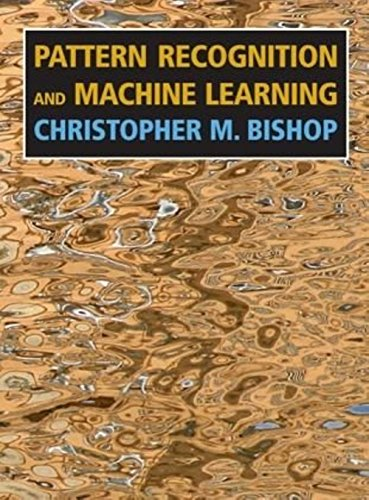
\includegraphics[width=0.25\linewidth]{figs/bishop}
	\caption{The front cover of \cite{bishop_pattern_2011}.}
	\label{fig:duda}
\end{figure}
\end{abstract}

\clearpage

{\small \tableofcontents}


\clearpage
\section{Chapter notes}

% ----------------------------------------------------------------------------
\subsection{Introduction}
\begin{easylist}[itemize]
	\ListProperties(Space=\listSpace, Space*=\listSpace, Numbers1=l, FinalMark1={)})
	# sdf
\end{easylist}

% ----------------------------------------------------------------------------
\subsection{Probability Distributions}
\begin{easylist}[itemize]
	\ListProperties(Space=\listSpace, Space*=\listSpace, Numbers1=l, FinalMark1={)})
	# sdf
\end{easylist}

% ----------------------------------------------------------------------------
\subsection{Linear Models for Regression}
\begin{easylist}[itemize]
	\ListProperties(Space=\listSpace, Space*=\listSpace, Numbers1=l, FinalMark1={)})
	# sdf
\end{easylist}

% ----------------------------------------------------------------------------
\subsection{Linear Models for Classification}
\begin{easylist}[itemize]
	\ListProperties(Space=\listSpace, Space*=\listSpace, Numbers1=l, FinalMark1={)})
	# sdf
\end{easylist}

% ----------------------------------------------------------------------------
\subsection{Neural networks}
\begin{easylist}[itemize]
	\ListProperties(Space=\listSpace, Space*=\listSpace, Numbers1=l, FinalMark1={)})
	# sdf
\end{easylist}

% ----------------------------------------------------------------------------
\subsection{Kernel methods}
\begin{easylist}[itemize]
	\ListProperties(Space=\listSpace, Space*=\listSpace, Numbers1=l, FinalMark1={)})
	# sdf
\end{easylist}

% ----------------------------------------------------------------------------
\subsection{Sparse Kernel Machines}
\begin{easylist}[itemize]
	\ListProperties(Space=\listSpace, Space*=\listSpace, Numbers1=l, FinalMark1={)})
	# sdf
\end{easylist}

% ----------------------------------------------------------------------------
\subsection{Graphical Models}
\begin{easylist}[itemize]
	\ListProperties(Space=\listSpace, Space*=\listSpace, Numbers1=l, FinalMark1={)})
	# sdf
\end{easylist}

% ----------------------------------------------------------------------------
\subsection{Mixture Models and EM}
\begin{easylist}[itemize]
	\ListProperties(Space=\listSpace, Space*=\listSpace, Numbers1=l, FinalMark1={)})
	# sdf
\end{easylist}

% ----------------------------------------------------------------------------
\subsection{Approximate Interference}
\begin{easylist}[itemize]
	\ListProperties(Space=\listSpace, Space*=\listSpace, Numbers1=l, FinalMark1={)})
	# sdf
\end{easylist}

% ----------------------------------------------------------------------------
\subsection{Sampling Methods}
\begin{easylist}[itemize]
	\ListProperties(Space=\listSpace, Space*=\listSpace, Numbers1=l, FinalMark1={)})
	# sdf
\end{easylist}

% ----------------------------------------------------------------------------
\subsection{Continuous Latent Variables}
\begin{easylist}[itemize]
	\ListProperties(Space=\listSpace, Space*=\listSpace, Numbers1=l, FinalMark1={)})
	# sdf
\end{easylist}

% ----------------------------------------------------------------------------
\subsection{Sequential Data}
\begin{easylist}[itemize]
	\ListProperties(Space=\listSpace, Space*=\listSpace, Numbers1=l, FinalMark1={)})
	# sdf
\end{easylist}

% ----------------------------------------------------------------------------
\subsection{Combining Models}
\begin{easylist}[itemize]
	\ListProperties(Space=\listSpace, Space*=\listSpace, Numbers1=l, FinalMark1={)})
	# sdf
\end{easylist}

% ----------------------------------------------------------------------------





\clearpage

\section{Chapter summaries}

% ----------------------------------------------------------------------------
\subsection{Introduction}
\begin{easylist}[itemize]
	\ListProperties(Space=\listSpace, Space*=\listSpace, Numbers1=l, FinalMark1={)})
	# sdf
\end{easylist}

% ----------------------------------------------------------------------------
\subsection{Probability Distributions}
\begin{easylist}[itemize]
	\ListProperties(Space=\listSpace, Space*=\listSpace, Numbers1=l, FinalMark1={)})
	# sdf
\end{easylist}

% ----------------------------------------------------------------------------
\subsection{Linear Models for Regression}
\begin{easylist}[itemize]
	\ListProperties(Space=\listSpace, Space*=\listSpace, Numbers1=l, FinalMark1={)})
	# sdf
\end{easylist}

% ----------------------------------------------------------------------------
\subsection{Linear Models for Classification}
\begin{easylist}[itemize]
	\ListProperties(Space=\listSpace, Space*=\listSpace, Numbers1=l, FinalMark1={)})
	# sdf
\end{easylist}

% ----------------------------------------------------------------------------
\subsection{Neural networks}
\begin{easylist}[itemize]
	\ListProperties(Space=\listSpace, Space*=\listSpace, Numbers1=l, FinalMark1={)})
	# sdf
\end{easylist}

% ----------------------------------------------------------------------------
\subsection{Kernel methods}
\begin{easylist}[itemize]
	\ListProperties(Space=\listSpace, Space*=\listSpace, Numbers1=l, FinalMark1={)})
	# sdf
\end{easylist}

% ----------------------------------------------------------------------------
\subsection{Sparse Kernel Machines}
\begin{easylist}[itemize]
	\ListProperties(Space=\listSpace, Space*=\listSpace, Numbers1=l, FinalMark1={)})
	# sdf
\end{easylist}

% ----------------------------------------------------------------------------
\subsection{Graphical Models}
\begin{easylist}[itemize]
	\ListProperties(Space=\listSpace, Space*=\listSpace, Numbers1=l, FinalMark1={)})
	# sdf
\end{easylist}

% ----------------------------------------------------------------------------
\subsection{Mixture Models and EM}
\begin{easylist}[itemize]
	\ListProperties(Space=\listSpace, Space*=\listSpace, Numbers1=l, FinalMark1={)})
	# sdf
\end{easylist}

% ----------------------------------------------------------------------------
\subsection{Approximate Interference}
\begin{easylist}[itemize]
	\ListProperties(Space=\listSpace, Space*=\listSpace, Numbers1=l, FinalMark1={)})
	# sdf
\end{easylist}

% ----------------------------------------------------------------------------
\subsection{Sampling Methods}
\begin{easylist}[itemize]
	\ListProperties(Space=\listSpace, Space*=\listSpace, Numbers1=l, FinalMark1={)})
	# sdf
\end{easylist}

% ----------------------------------------------------------------------------
\subsection{Continuous Latent Variables}
\begin{easylist}[itemize]
	\ListProperties(Space=\listSpace, Space*=\listSpace, Numbers1=l, FinalMark1={)})
	# sdf
\end{easylist}

% ----------------------------------------------------------------------------
\subsection{Sequential Data}
\begin{easylist}[itemize]
	\ListProperties(Space=\listSpace, Space*=\listSpace, Numbers1=l, FinalMark1={)})
	# sdf
\end{easylist}

% ----------------------------------------------------------------------------
\subsection{Combining Models}
\begin{easylist}[itemize]
	\ListProperties(Space=\listSpace, Space*=\listSpace, Numbers1=l, FinalMark1={)})
	# sdf
\end{easylist}

% ----------------------------------------------------------------------------
















\clearpage
\section{Solutions}

% ----------------------------------------------------------------------------
\subsection{Introduction}
\subsubsection*{Problem X.Y}
\begin{easylist}[enumerate]
	\ListProperties(Space=\listSpace, Space*=\listSpace, Numbers1=l, FinalMark1={)})
	# sdf
\end{easylist}

% ----------------------------------------------------------------------------
\subsection{Probability Distributions}
\subsubsection*{Problem X.Y}
\begin{easylist}[enumerate]
	\ListProperties(Space=\listSpace, Space*=\listSpace, Numbers1=l, FinalMark1={)})
	# sdf
\end{easylist}

% ----------------------------------------------------------------------------
\subsection{Linear Models for Regression}
\subsubsection*{Problem X.Y}
\begin{easylist}[enumerate]
	\ListProperties(Space=\listSpace, Space*=\listSpace, Numbers1=l, FinalMark1={)})
	# sdf
\end{easylist}

% ----------------------------------------------------------------------------
\subsection{Linear Models for Classification}
\subsubsection*{Problem X.Y}
\begin{easylist}[enumerate]
	\ListProperties(Space=\listSpace, Space*=\listSpace, Numbers1=l, FinalMark1={)})
	# sdf
\end{easylist}

% ----------------------------------------------------------------------------
\subsection{Neural networks}
\subsubsection*{Problem X.Y}
\begin{easylist}[enumerate]
	\ListProperties(Space=\listSpace, Space*=\listSpace, Numbers1=l, FinalMark1={)})
	# sdf
\end{easylist}

% ----------------------------------------------------------------------------
\subsection{Kernel methods}
\subsubsection*{Problem X.Y}
\begin{easylist}[enumerate]
	\ListProperties(Space=\listSpace, Space*=\listSpace, Numbers1=l, FinalMark1={)})
	# sdf
\end{easylist}

% ----------------------------------------------------------------------------
\subsection{Sparse Kernel Machines}
\subsubsection*{Problem X.Y}
\begin{easylist}[enumerate]
	\ListProperties(Space=\listSpace, Space*=\listSpace, Numbers1=l, FinalMark1={)})
	# sdf
\end{easylist}

% ----------------------------------------------------------------------------
\subsection{Graphical Models}
\subsubsection*{Problem X.Y}
\begin{easylist}[enumerate]
	\ListProperties(Space=\listSpace, Space*=\listSpace, Numbers1=l, FinalMark1={)})
	# sdf
\end{easylist}

% ----------------------------------------------------------------------------
\subsection{Mixture Models and EM}
\subsubsection*{Problem X.Y}
\begin{easylist}[enumerate]
	\ListProperties(Space=\listSpace, Space*=\listSpace, Numbers1=l, FinalMark1={)})
	# sdf
\end{easylist}

% ----------------------------------------------------------------------------
\subsection{Approximate Interference}
\subsubsection*{Problem X.Y}
\begin{easylist}[enumerate]
	\ListProperties(Space=\listSpace, Space*=\listSpace, Numbers1=l, FinalMark1={)})
	# sdf
\end{easylist}

% ----------------------------------------------------------------------------
\subsection{Sampling Methods}
\subsubsection*{Problem X.Y}
\begin{easylist}[enumerate]
	\ListProperties(Space=\listSpace, Space*=\listSpace, Numbers1=l, FinalMark1={)})
	# sdf
\end{easylist}

% ----------------------------------------------------------------------------
\subsection{Continuous Latent Variables}
\subsubsection*{Problem X.Y}
\begin{easylist}[enumerate]
	\ListProperties(Space=\listSpace, Space*=\listSpace, Numbers1=l, FinalMark1={)})
	# sdf
\end{easylist}

% ----------------------------------------------------------------------------
\subsection{Sequential Data}
\subsubsection*{Problem X.Y}
\begin{easylist}[enumerate]
	\ListProperties(Space=\listSpace, Space*=\listSpace, Numbers1=l, FinalMark1={)})
	# sdf
\end{easylist}

% ----------------------------------------------------------------------------
\subsection{Combining Models}
\subsubsection*{Problem X.Y}
\begin{easylist}[enumerate]
	\ListProperties(Space=\listSpace, Space*=\listSpace, Numbers1=l, FinalMark1={)})
	# sdf
\end{easylist}

% ----------------------------------------------------------------------------



































\bibliographystyle{apalike}%alpha, apalike is also good
\bibliography{../bibliography}


\end{document}
